% !TEX TS-program = pdflatex
% !TEX encoding = UTF-8 Unicode

% This is a simple template for a LaTeX document using the "article" class.
% See "book", "report", "letter" for other types of document.

\documentclass[11pt]{article} % use larger type; default would be 10pt

\usepackage[utf8]{inputenc} % set input encoding (not needed with XeLaTeX)

%%% Examples of Article customizations
% These packages are optional, depending whether you want the features they provide.
% See the LaTeX Companion or other references for full information.

%%% PAGE DIMENSIONS
\usepackage{geometry} % to change the page dimensions
\geometry{a4paper} % or letterpaper (US) or a5paper or....
% \geometry{margin=2in} % for example, change the margins to 2 inches all round
% \geometry{landscape} % set up the page for landscape
%   read geometry.pdf for detailed page layout information

\usepackage{graphicx} % support the \includegraphics command and options

% \usepackage[parfill]{parskip} % Activate to begin paragraphs with an empty line rather than an indent

%%% PACKAGES
\usepackage{booktabs} % for much better looking tables
\usepackage{array} % for better arrays (eg matrices) in maths
%\usepackage{paralist} % very flexible & customisable lists (eg. enumerate/itemize, etc.)
\usepackage{verbatim} % adds environment for commenting out blocks of text & for better verbatim
\usepackage{subfig} % make it possible to include more than one captioned figure/table in a single float
% These packages are all incorporated in the memoir class to one degree or another...

%%% HEADERS & FOOTERS
\usepackage{fancyhdr} % This should be set AFTER setting up the page geometry
\pagestyle{fancy} % options: empty , plain , fancy
\renewcommand{\headrulewidth}{0pt} % customise the layout...
\lhead{}\chead{}\rhead{}
\lfoot{}\cfoot{\thepage}\rfoot{}

%%% SECTION TITLE APPEARANCE
\usepackage{sectsty}
\allsectionsfont{\sffamily\mdseries\upshape} % (See the fntguide.pdf for font help)
% (This matches ConTeXt defaults)

%%% ToC (table of contents) APPEARANCE
\usepackage[nottoc,notlof,notlot]{tocbibind} % Put the bibliography in the ToC
\usepackage[titles,subfigure]{tocloft} % Alter the style of the Table of Contents
\renewcommand{\cftsecfont}{\rmfamily\mdseries\upshape}
\renewcommand{\cftsecpagefont}{\rmfamily\mdseries\upshape} % No bold!

%%% END Article customizations

\usepackage[spanish]{babel}
\usepackage{listings} 
%%% The "real" document content comes below...

\title{JS}
%\date{} % Activate to display a given date or no date (if empty),
         % otherwise the current date is printed 

\begin{document}
\maketitle
%\tableofcontents % No hace falta un TOC en un artículo corto

\section{Introducción}
La presente investigación es sobre el lenguaje de programación JavaSript  (lenguaje interpretado  dialecto del estándar ECMAScript) definido como un lenguaje orientado a objetos.\\
\\La característica principal de JavaSript es su simplicidad y manejabilidad.\\
\\Para conocer más sobre este lenguaje de programación veremos las características más importantes,  como surgió, los requisitos para su correcta instalación y la forma más sencilla de aprender JavaScript. \\
\\La investigación se realiza por el interés de aprender sobre un nuevo lenguaje el cual nos aporte más conocimientos sobre el amplio mundo de la programación.\\
\\Es necesario recalcar que existen dos tipos de JavaScript: El que se denomina Navigator JavaScript que es el JavaScript propiamente dicho que es el que se ejecuta en el cliente. Pero además un JavaScript denominado LiveWire Javascript que se ejecuta en el servidor.\\
\\ \\

OBJETIVOS:
\\ \\
\\Analizar que es JavaScript por quienes puede ser utilizado, su manejo, y características.
Diferenciar para que específicamente se utilicen los dos tipos que poseen JavaScript y las diferencias de Java vs JavaScript
Aprender la correcta instalación y uso.\\

\section{Características}
{\bfseries JavaScript} es un lenguaje muy simple y manejable. Cuenta con las siguientes características:\\\\
Variables (no se necesita declaración de tipo de dato) : n=2; o var nombre ;\\
Condiciones: if (i<10){.....} else{}\\
Ciclos: for (j=0; j<10; j++){......}\\
Funciones definidas por el usuario o propias del lenguaje\\
Comentarios: // Esto es un comentario de una línea\\
/*Comentario\\
multilinea*/   \\
Permite la programación orientada a objeto: function miFuncion(a,b){..........} \\
Permite concatenar:\\
var hello = "Hello "; \\
var world = "world!";\\
var n = hello.concat(world);

\section{TUTORIAL DE INSTALACION}
 Desde que los navegadores incluyen el Javascript, no necesitamos el Java Runtime Environment (JRE), para que se ejecute.
\\  \\
Como habilitar JavaScrpt en tu navegador 
Ahora ya todas las páginas web contienen  JavaScript, un lenguaje de programación que se ejecuta en el navegador web del visitante. \\\\
Con esto se crean páginas específicas en las páginas web y si es desactivada o deja de funcionar por cualquier motivo la página web puede verse limitada o no quedar disponible.
\\\\
Veremos como habilitar(activar) JavaScript en cuatro de los navegadores mas utilizados:
\newline
\newline* Google Chrome
\newline* Mozilla Firefox
\newline* Internet Explorer
\newline
* Opera

\subsection{Google Chrome}
Aquí veremos como activar JS en uno de los navegadores mas populares y utilizados por los usuarios que es Google Chrome 

\begin{figure}
\begin{center}
\begin{center}
Navegar google Chrome
\end{center}

\includegraphics[height=3 cm, width=3 cm] {imagenes/chrome.jpg}

\ Imagen 1
\ label { http://www.enable-javascript.com/images/chrome.gif }
\newline

\begin{center}

\bf PASO 1 
 En el navegador web, haz click en el menú ''Customize and control Google Chrome'' 
y luego selecciona "Settings".
\end{center}

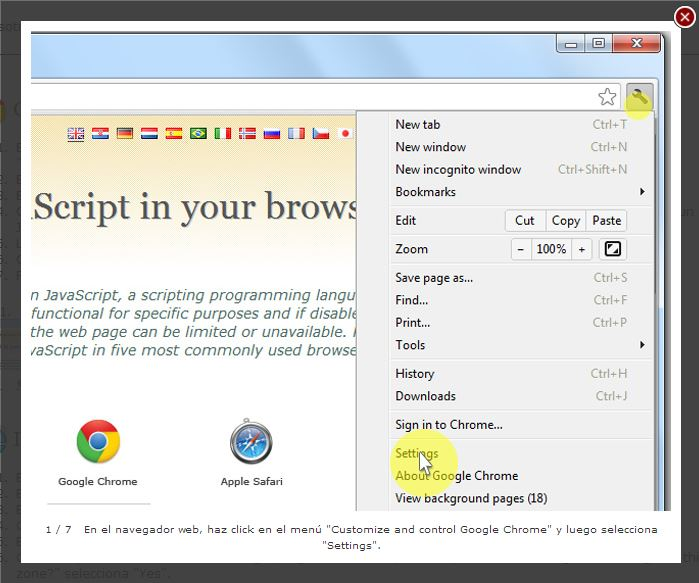
\includegraphics[height=8cm, width=8 cm] {imagenes/chrome 01.jpg}
\newline
\  Imagen 2
\ label { http://www.enable-javascript.com/images/chrome.gif }
\newline

\begin{center}

\bf PASO 2
En la sección "Settings" haz click en la 
opción "Show advanced settings..."
\end{center}
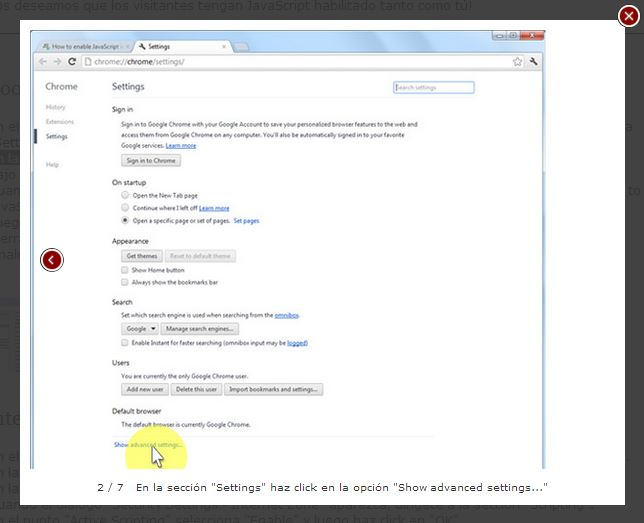
\includegraphics[height=8cm, width=8 cm] {imagenes/chrome 02.jpg}
\newline
\  Imagen 3
\ label { http://www.enable-javascript.com/images/chrome.gif }
\newline



\end{center}
\end{figure}

\begin{figure}
\begin{center}
\begin{center}
\bf PASO 3
Bajo la sección "Privacy" haz click en la opción 
``content settings..`` ... (recommended)
\newline
\end{center}
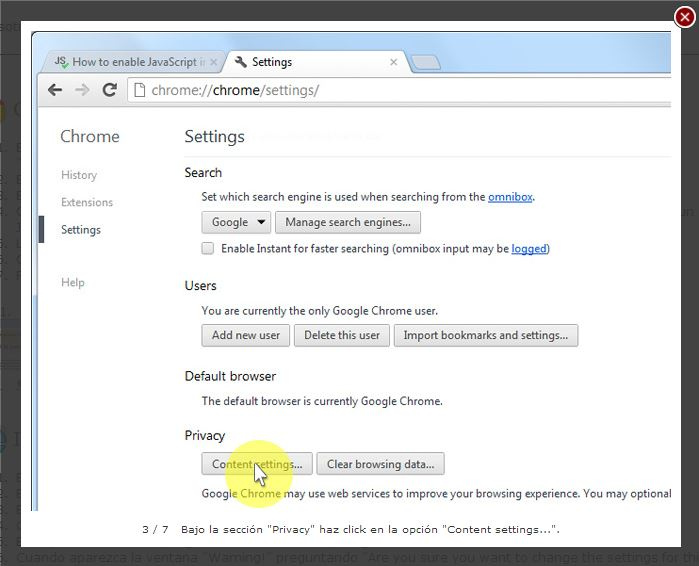
\includegraphics[height=8 cm, width=8 cm] {imagenes/chrome 03.jpg}
\newline
\ Imagen 4
\ label { http://www.enable-javascript.com/images/chrome.gif }
\newline


\begin{center}
\bf PASO 4
Cuando la ventana aparezca, dirigirse a la sección ``JavaScript``  y seleccionar la opción ``Allow all sites to run JavaScript (recommended)``
\newline
\end{center}

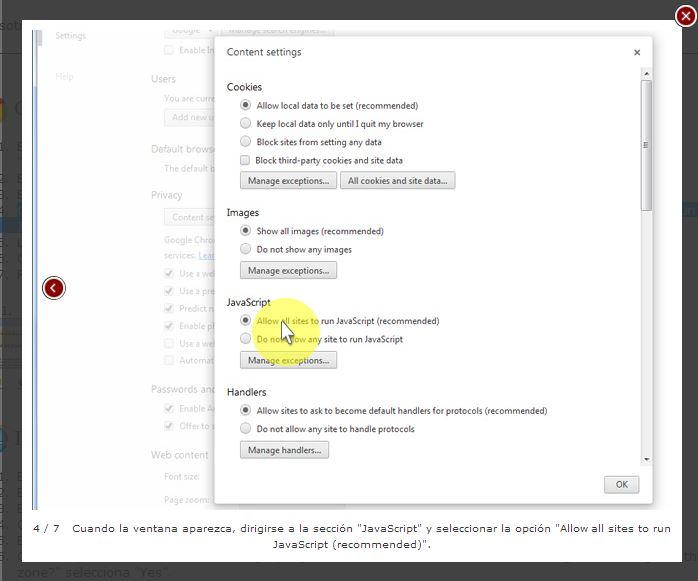
\includegraphics[height=8cm, width=8 cm] {imagenes/chrome 04.jpg}
\newline
\ Imagen 5

\ label { http://www.enable-javascript.com/images/chrome.gif }
\end{center}
\end{figure}

\begin{figure}
\begin{center}
\begin{center}
\bf PASO 5
Luego haz click en el botón ``OK`` para cerrar la ventana. (recommended)
\newline
\end{center}

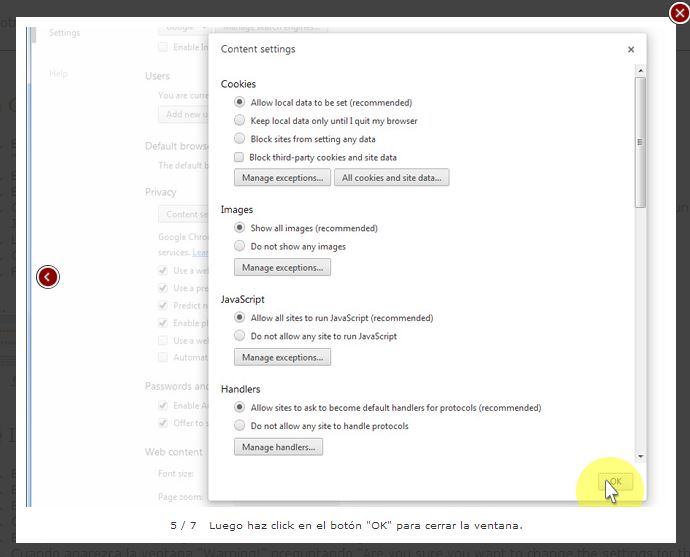
\includegraphics[height=8cm, width=8 cm] {imagenes/chrome 05.jpg}
\newline
\newline
\ Imagen 6
\ label { http://www.enable-javascript.com/images/chrome.gif }
\newline
\begin{center}
\bf PASO 6 Cierra la pestaña "Settings".
\end{center}

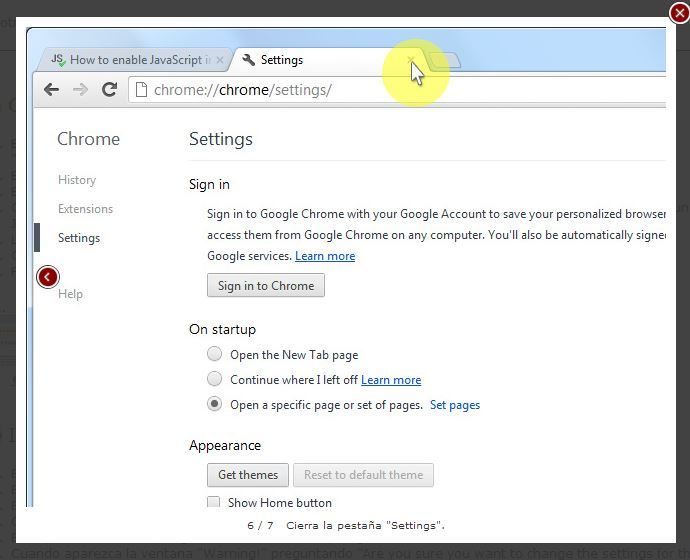
\includegraphics[height=8cm, width=8 cm] {imagenes/chrome 06.jpg}
\newline
\newline
\ Imagen 7
\ label { http://www.enable-javascript.com/images/chrome.gif }


\end{center}
\end{figure}


\begin{figure}
\begin{center}
\begin{center}
\bf PASO 7
Finalmente haz click en el botón ``Reload this page`` del navegador web para refrescar la página.
\newline
\end{center}

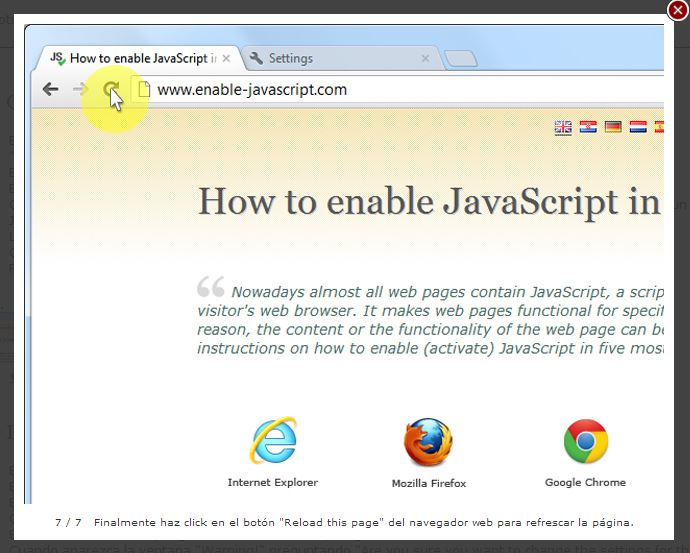
\includegraphics[height=8cm, width=8 cm] {imagenes/chrome 07.jpg}
\newline
\ Imagen 8
\ label { http://www.enable-javascript.com/images/chrome.gif }
\end{center}
\end{figure}


\newpage

\subsection{Mozilla FireFox}

Ahora mostraremos los pasos para otro navegador popular como el Mozilla FireFox
\newline
\begin{figure}
\begin{center}
\begin{center}
Navegar Mozilla Firefox

\end{center}
\begin{center}

\includegraphics[height=3 cm, width=3 cm] {imagenes/firefox.jpg}
\end{center}


\ Imagen 9
\ label {http://www.enable-javascript.com/images/firefox.gif }

\begin{center}
\bf PASO 1 
En el navegador web, has click en el menú ``Firefox`` y luego selecciona el item ``Tools``
y luego selecciona ``Settings``
\end{center}

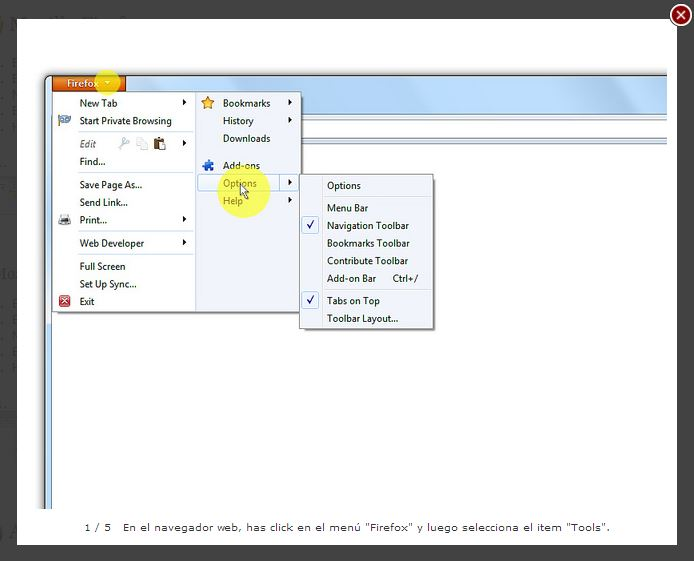
\includegraphics[height=8 cm, width=8 cm] {imagenes/firefox 01.jpg}
\newline
\newline
\ Imagen 10
\ label {http://www.enable-javascript.com/images/firefox.gif }

\begin{center}
\bf PASO 2
En la ventana ``Options`` selecciona la pestaña ``Content``.
\end{center}

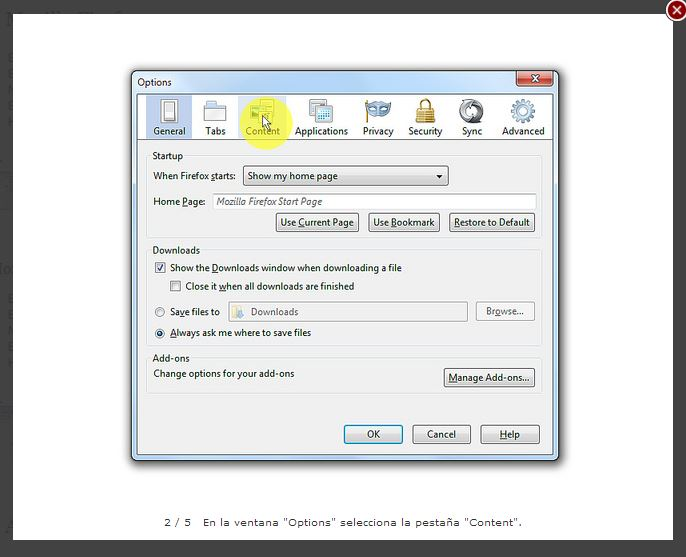
\includegraphics[height=8 cm, width=8 cm] {imagenes/firefox 02.jpg}
\newline
\newline
\ Imagen 11
\ label {http://www.enable-javascript.com/images/firefox.gif }

\end{center}
\end{figure}

\begin{figure}
\begin{center}

\begin{center}
\bf PASO 3
Marca la casilla ``Enable JavaScript``
\newline
\end{center}
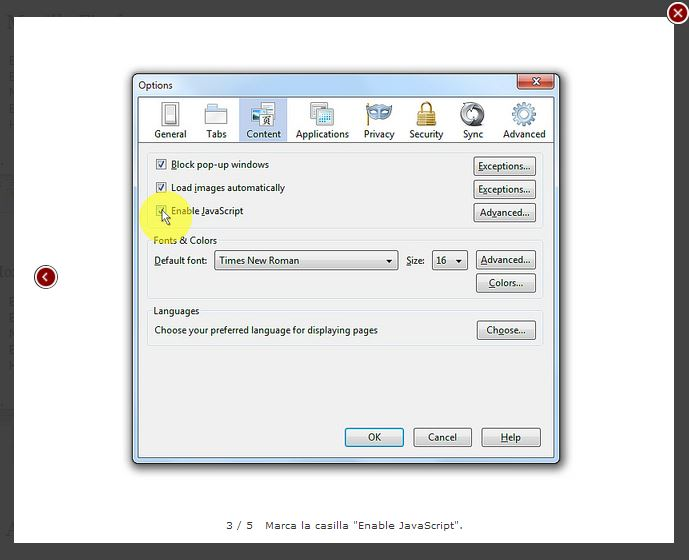
\includegraphics[height=8 cm, width=8 cm] {imagenes/firefox 03.jpg}
\newline
\newline
\ Imagen 12
\ label {http://www.enable-javascript.com/images/firefox.gif }

\begin{center}
\bf PASO 4
En la ventana `` Options`` (ya abierta) haz click en el botón ``OK`` para cerrarla.
\end{center}
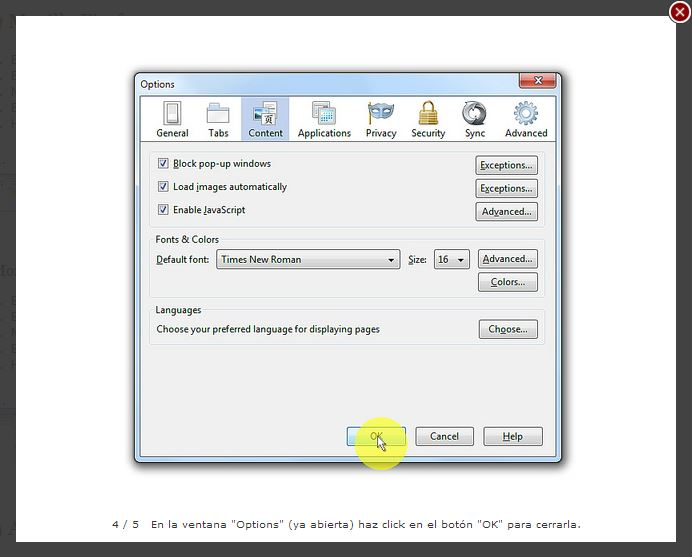
\includegraphics[height=8 cm, width=8 cm] {imagenes/firefox 04.jpg}
\newline
\newline
\ Imagen 13
\ label {http://www.enable-javascript.com/images/firefox.gif }

\end{center}
\end{figure}

\begin{figure}
\begin{center}
\begin{center}
\bf PASO 5
Haz click en el botón ``Reload current page`` del navegador para recargar la página.
\newline
\end{center}
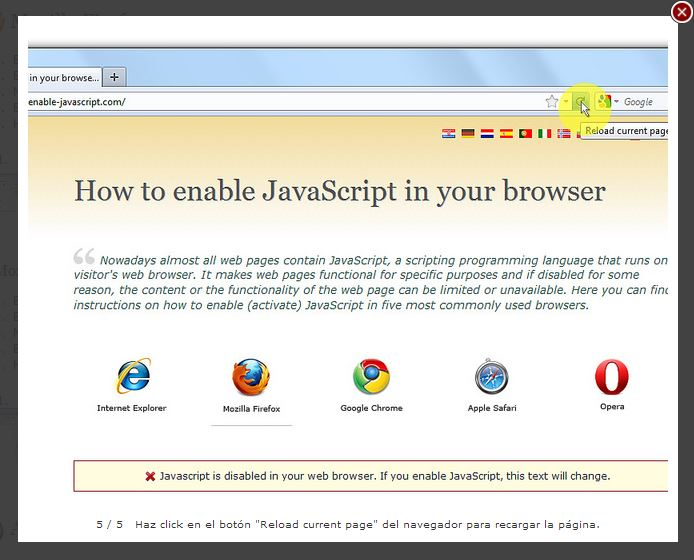
\includegraphics[height=8 cm, width=8 cm] {imagenes/firefox 05.jpg}
\newline
\newline
\ Imagen 14
\ label {http://www.enable-javascript.com/images/firefox.gif }

\end{center}
\end{figure}

\newpage
\subsection{Internet Explorer}

Pasos para activar JavaScript en internet explorer

\begin{figure}
\begin{center}
\begin{center}
Navegar Internet Explorer

\end{center}
\begin{center}

\includegraphics[height=3 cm, width=3 cm] {imagenes/explorer.jpg}
\end{center}

\ Imagen 15
\ label {http://www.enable-javascript.com/images/ie9.gif }
\newline

\begin{center}
\bf PASO 1
En el menú del navegador web, has click en el icono ``Tools`` y selecciona la opción ``Internet Options``
\end{center}
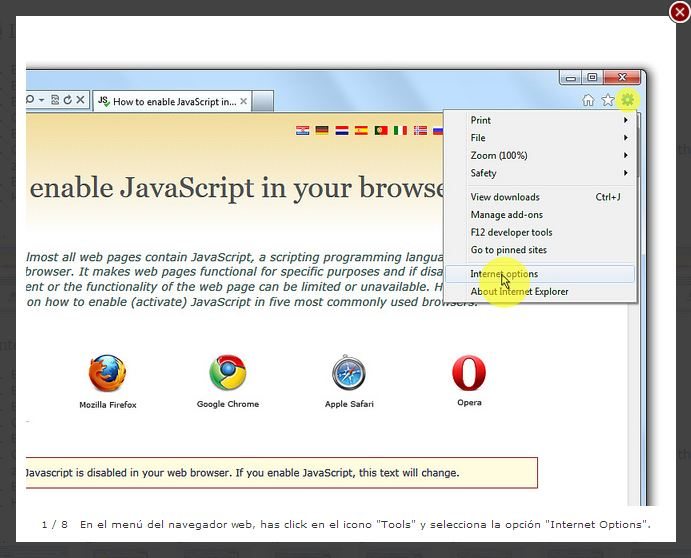
\includegraphics[height=8 cm, width=8 cm] {imagenes/explorer 01.jpg}
\newline
\newline
\ Imagen 16
\ label {http://www.enable-javascript.com/images/ie9.gif }

\begin{center}
\bf PASO 2
En la ventana ``Internet Options`` selecciona la pestaña ``Security``.
\end{center}

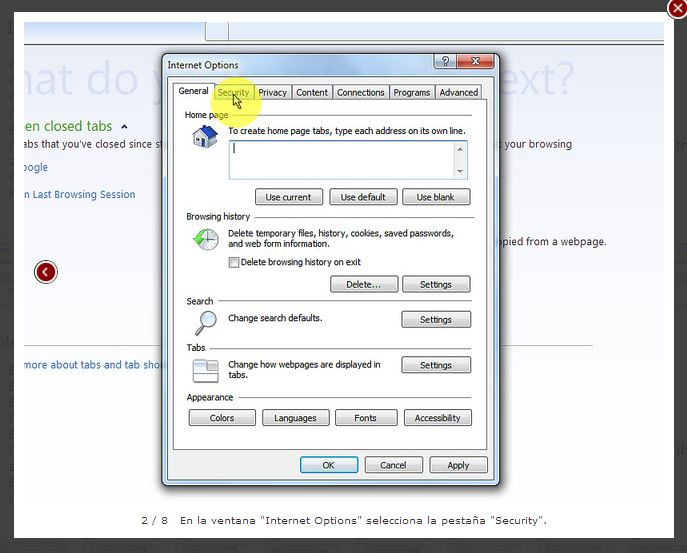
\includegraphics[height=8 cm, width=8 cm] {imagenes/explorer 02.jpg}
\newline
\newline
\ Imagen 17
\ label {http://www.enable-javascript.com/images/ie9.gif }

\end{center}
\end{figure}

\begin{figure}
\begin{center}

\begin{center}
\bf PASO 3
En la pestaña ``Security`` haz click en el botón ``Custom level...``
\end{center}
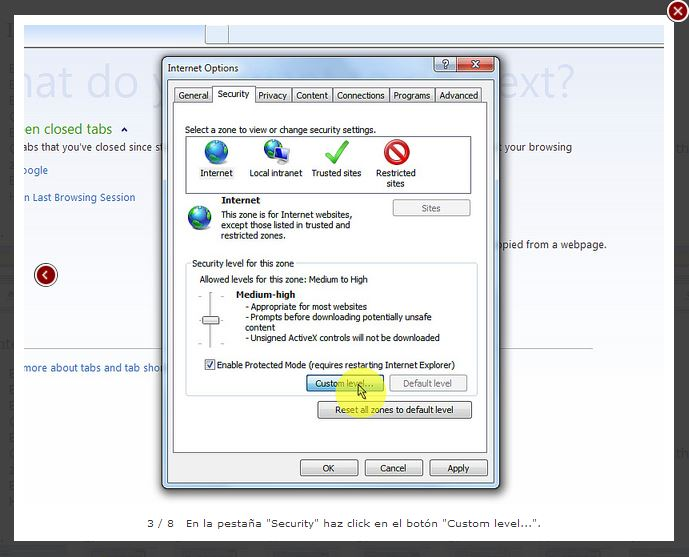
\includegraphics[height=8 cm, width=8 cm] {imagenes/explorer 03.jpg}
\newline
\newline
\ Imagen 18 
\ label {http://www.enable-javascript.com/images/ie9.gif }
\newline
\begin{center}
\bf PASO 4
Cuando el diálogo ``Security Settings - Internet Zone`` aparezca, dirígete a la sección ``Scripting``
\end{center}
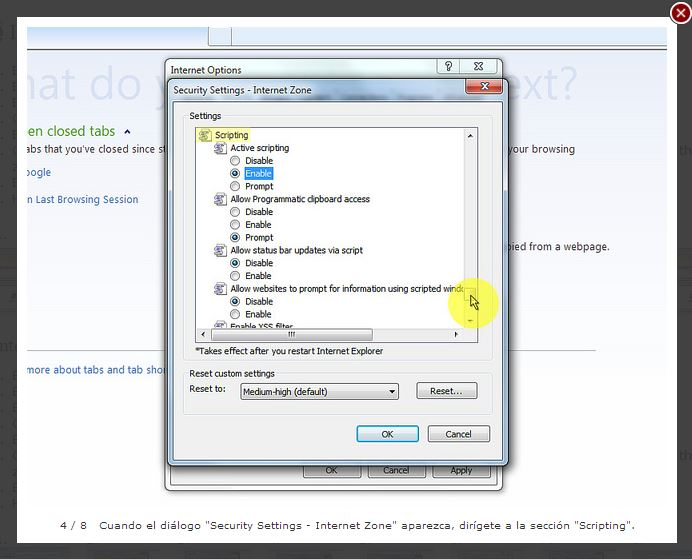
\includegraphics[height=8 cm, width=8 cm] {imagenes/explorer 04.jpg}
\newline
\newline
\ Imagen 19
\ label {http://www.enable-javascript.com/images/ie9.gif }

\end{center}
\end{figure}


\begin{figure}
\begin{center}

\begin{center}
\bf PASO 5
En el punto ``Active Scripting`` selecciona ``Enable`` y luego haz click en ``OK``
\end{center}
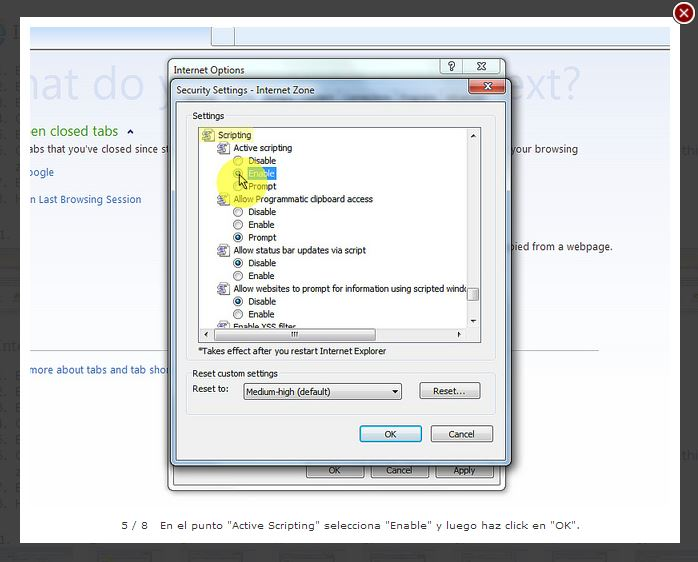
\includegraphics[height=8 cm, width=8 cm] {imagenes/explorer 05.jpg}
\newline
\newline
\ Imagen 20
\ label {http://www.enable-javascript.com/images/ie9.gif }
\newline

\begin{center}
\bf PASO 6
Cuando aparezca la ventana ``Warning!``  preguntando  ``Are you sure you want to change the settings for this zone?  selecciona ``Yes``
\end{center}
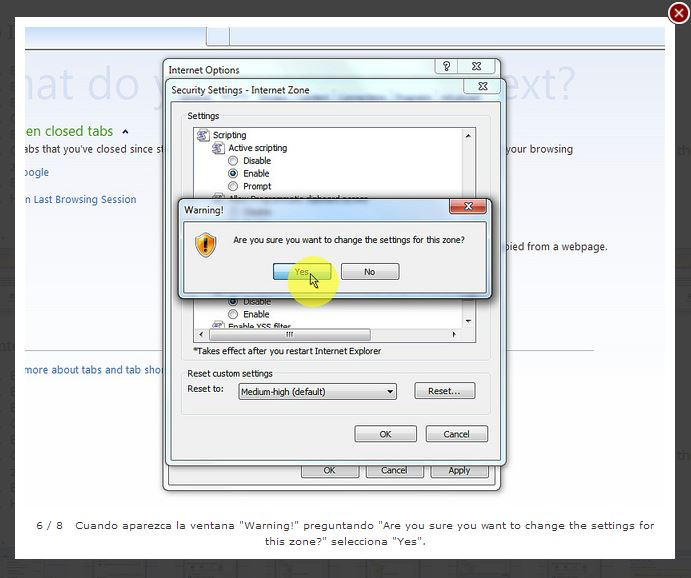
\includegraphics[height=8 cm, width=8 cm] {imagenes/explorer 06.jpg}
\newline
\newline
\ Imagen 21
\ label {http://www.enable-javascript.com/images/ie9.gif }

\end{center}
\end{figure}


\begin{figure}
\begin{center}

\begin{center}
\bf PASO 7
En la ventana ``Internet Options`` haz click en el botón ``OK``para cerrarla.
\end{center}
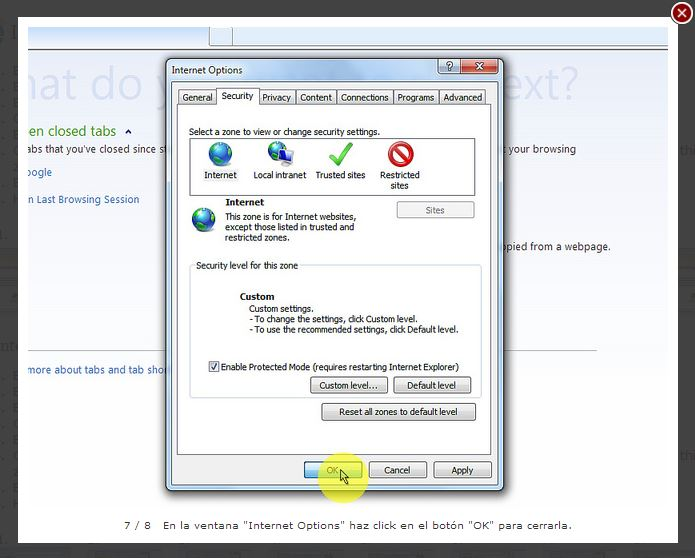
\includegraphics[height=8 cm, width=8 cm] {imagenes/explorer 07.jpg}
\newline
\newline
\ Imagen 22
\ label {http://www.enable-javascript.com/images/ie9.gif }

\begin{center}
\bf PASO 8
Haz click en el botón ``Refresh`` del navegador para recargar la página.
\end{center}

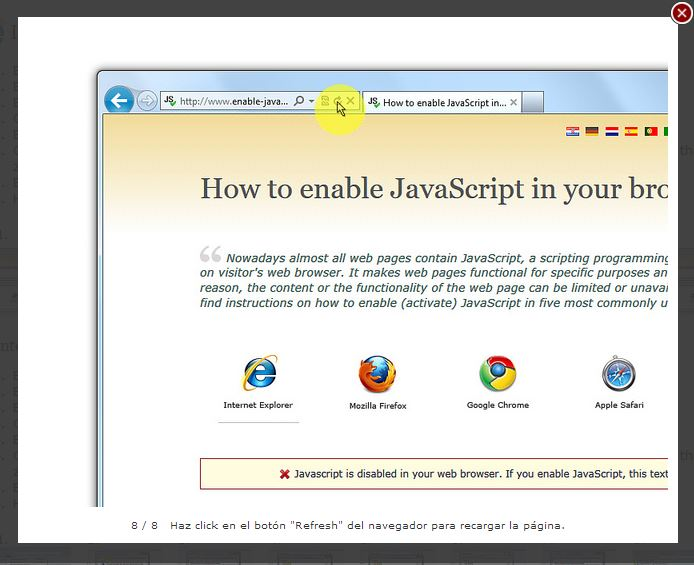
\includegraphics[height=8 cm, width=8 cm] {imagenes/explorer 08.jpg}
\newline
\newline
\ Imagen 23
\ label {http://www.enable-javascript.com/images/ie9.gif }

\end{center}
\end{figure}


\newpage
\subsection{Navegador Opera}

Pasos para activar JavaScript en navegador Opera

\begin{figure}
\begin{center}
\begin{center}
Navegar Opera

\end{center}
\begin{center}
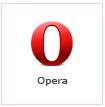
\includegraphics[height=3 cm, width=3 cm] {imagenes/opera.jpg}
\end{center}

\ Imagen 24
\ label {http://www.enable-javascript.com/images/opera.gif}
\newline

\begin{center}
\bf PASO 1
a) Haz click en el botón ``Menu`` del navegador web. En las opciones que aparecen, dirígite a ``Settings``, luego a ``Quick preferences`` y marca la casilla ``Enable JavaScript``.
\end{center}
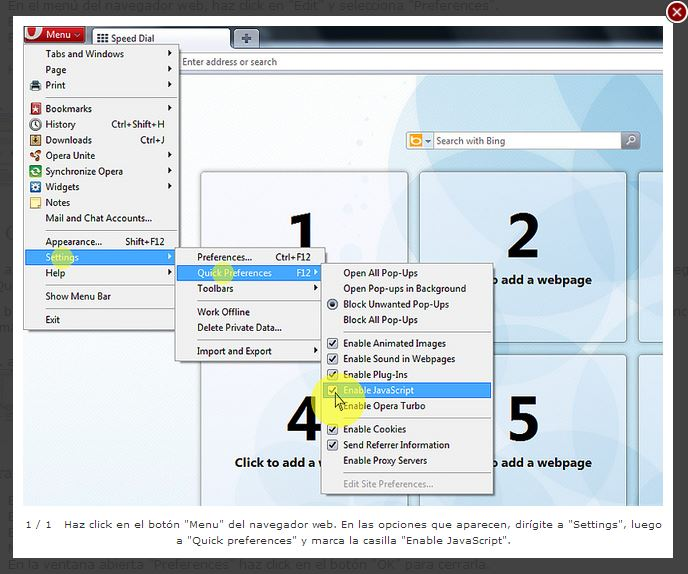
\includegraphics[height=8 cm, width=8 cm] {imagenes/opera 01.jpg}
\newline
\newline
\ Imagen 25
\ label {http://www.enable-javascript.com/images/opera.gif}

\end{center}
\end{figure}

\begin{figure}
\begin{center}

\begin{center}
\bf PASO 1
 b) Si el "Menu bar" se encuentra, haz click en la opción ``Tools`` del navegador web, luego a ``Quick preferences`` y marca la casilla ``Enable JavaScript``.
\end{center}

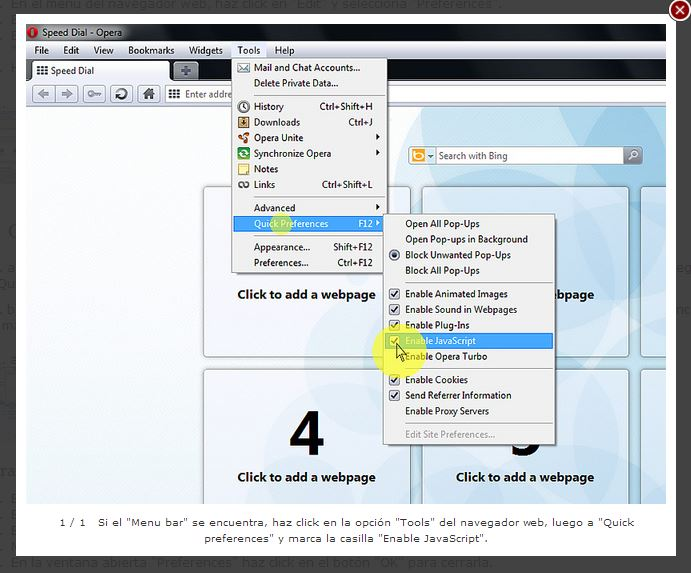
\includegraphics[height=8 cm, width=8 cm] {imagenes/opera 02.jpg}
\newline
\newline
\ Imagen 26
\ label {http://www.enable-javascript.com/images/opera.gif}

\end{center}
\end{figure}

\lstset{language=Pascal}          % Set your language (you can change the language for each code-block optionally)





\end{document}